\documentclass[nobib]{tufte-handout}
% nobib: use natbib + bibtex so citations still appear as margin notes via \cite

\usepackage[round]{natbib}
\setcitestyle{authoryear}
\usepackage{amsmath,amssymb}
\usepackage{booktabs}
\usepackage{graphicx}
\usepackage{siunitx}
\sisetup{group-separator={,},per-mode=symbol}
\usepackage{xcolor}
\definecolor{econred}{HTML}{E3120B}
\usepackage{microtype}

% citations as sidenotes (tufte style) while keeping a reference list
\renewcommand{\cite}[2][]{\sidenote{\citet{#2}\ifx&#1&\else, #1\fi.}}

\title{Water hammer in domestic hot water pipes}
\author{The physics behind the waterhammer screening model}
\date{October 2026}

\newcommand{\dd}{\mathrm{d}}

\begin{document}
\maketitle

\begin{abstract}
\noindent When a tap or appliance valve shuts, the moving column of water in the pipe behind it is brought to rest and its momentum appears as a pressure wave.
This note sets out the physics the \texttt{waterhammer} model uses to decide whether a domestic hot water branch needs protection: the wave speed in an elastic pipe, the Joukowsky and Michaud surge estimates, a method-of-characteristics simulation, column separation and the sizing of a gas-cushion arrester.
It closes with the acceptance limits and a worked example.
The Python package and the Excel workbook implement exactly these equations; the two agree to machine precision.
\end{abstract}

\section{The mechanism}

Consider a pipe of bore $D$ and length $L$ fed from a point where the pressure stays nearly constant (a larger main, a manifold, a hot water cylinder or an expansion vessel: the \emph{reflection point}) and ending at a valve.
Water flows at mean velocity $v = Q/A$, where $A = \pi D^2/4$.

When the valve shuts, the layer of water next to it stops first.
Its pressure rises, compressing the water and stretching the pipe wall, and the region of raised pressure spreads upstream at the \emph{wave speed} $a$.
When the front reaches the reflection point after $L/a$, the pipe is entirely at rest and over-pressurised.
Water then flows back out into the reflection point and a relief wave travels down to the valve, arriving at time
\begin{equation}
  T_c = \frac{2L}{a},
\end{equation}
the \emph{critical time}.\marginnote{A \SI{10}{m} copper run has $T_c \approx \SI{15}{ms}$; the same run in PE-X has $T_c \approx \SI{70}{ms}$.}
Without friction the cycle would repeat for ever, alternating high and low pressure at the valve with period $4L/a$.
Friction damps it, and in practice so do trapped air, flexible hoses and fittings that move.

\section{Surge from a rapid closure: Joukowsky}

Take a control volume around the wave front, which moves upstream at $a$ (relative to the pipe, as $a \gg v$).
In time $\delta t$ the front sweeps a length $a\,\delta t$ and brings a mass $\rho A a\,\delta t$ from velocity $v$ to $v - \Delta v$.
The impulse needed comes from the pressure step $\Delta p$ acting on the area $A$:
\begin{equation}
  \Delta p\,A\,\delta t = \rho A a\,\delta t\,\Delta v
  \quad\Longrightarrow\quad
  \boxed{\Delta p = \rho\,a\,\Delta v}
  \label{eq:joukowsky}
\end{equation}
This is Joukowsky's equation.\cite{joukowsky1904}
It applies when the whole change of velocity happens before the first relief wave returns, that is when the valve's effective closure time $t_v \le T_c$.
Note that the surge does not depend on the length of the pipe or on the pressure already present.
\marginnote{In copper $\rho a \approx \SI{13}{bar}$ per \si{m/s}. A \SI{1}{m/s} flow stopped instantly gives \SI{13}{bar}, more than six times the \SI{2}{bar} limit.}

\section{Wave speed in an elastic pipe}

The wave speed follows from mass conservation across the front.
The water arriving in time $\delta t$, $\rho A v\,\delta t$, has to be stored in the length $a\,\delta t$ by compressing the water (bulk modulus $K$) and by stretching the pipe:
\begin{equation}
  v\,\delta t = a\,\delta t\left(\frac{\Delta p}{K} + \frac{\Delta A}{A}\right).
\end{equation}
For a pipe of wall thickness $e$ and Young's modulus $E$, the hoop strain gives $\Delta A / A = \psi\,\Delta p\,D/(E e)$, where $\psi$ accounts for axial restraint and wall thickness.
Combining this with Equation~\ref{eq:joukowsky} ($\Delta v = \Delta p/\rho a$) gives the Korteweg formula\cite[eq.~2.21]{wylie1993}
\begin{equation}
  \boxed{a = \sqrt{\frac{K/\rho}{1 + \psi\,\dfrac{K D}{E e}}}}
  \label{eq:wavespeed}
\end{equation}
For a thick-walled pipe with Poisson's ratio $\nu$, the restraint factor is
\begin{equation}
  \psi = 2\frac{e}{D}(1+\nu) + \frac{D}{D+e}\,\phi,
\end{equation}
with $\phi = 1-\nu^2$ for a pipe anchored against axial movement throughout (clipped or buried), $\phi = 1$ for a pipe free to move axially, and $\phi = 1-\nu/2$ for a pipe anchored at its upstream end only.
\marginnote{For thin pipes $\psi \to 1$ whatever the restraint, which is the textbook form of Equation~\ref{eq:wavespeed}.}
In a rigid pipe $a$ tends to the speed of sound in water, about \SI{1500}{m/s}.
Copper is stiff enough ($E \approx \SI{117}{GPa}$) to stay close to that value.
Plastics are a hundred times more flexible, so the pipe term dominates and $a$ falls to a few hundred metres per second (Figure~\ref{fig:wavespeed}).

\begin{figure}
  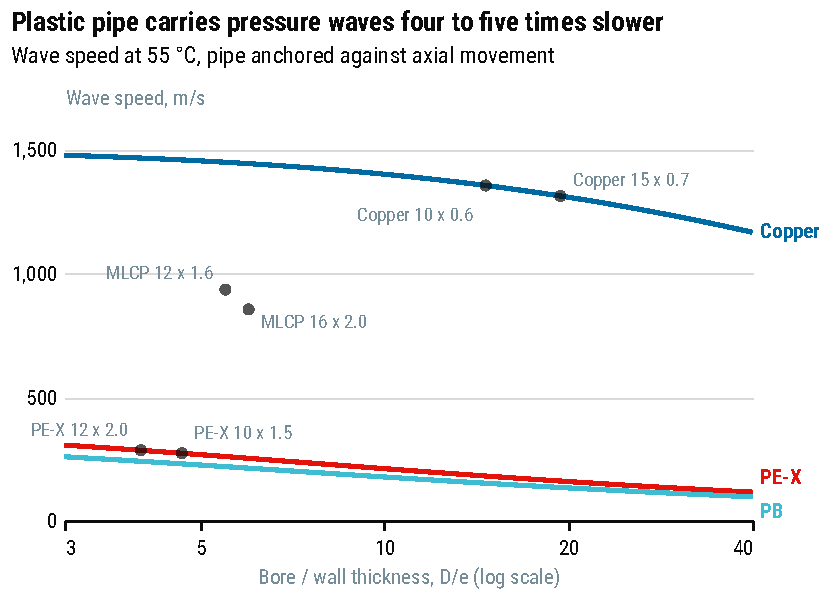
\includegraphics[width=\linewidth]{figures/wave_speed.pdf}
  \caption{Wave speed against bore-to-wall ratio at \SI{55}{\celsius}. The multilayer (MLCP) points assume a \SI{0.2}{mm} aluminium layer, with the wall's hoop stiffness taken as the thickness-weighted mean of aluminium and PE-RT.}
  \label{fig:wavespeed}
\end{figure}

\paragraph{Properties used.}
$K = \rho c^2$ is the isentropic bulk modulus, from the IAPWS-95 density and speed of sound $c$.\cite{iapws95}
$K$ peaks near \SI{50}{\celsius}, so hot water gives a slightly \emph{higher} surge than cold water in copper.
For plastics the relevant modulus is the short-term (dynamic) one, because the load lasts milliseconds.
It falls steeply with temperature: for PE-X the model uses \SI{0.70}{GPa} at \SI{20}{\celsius} and \SI{0.42}{GPa} at \SI{60}{\celsius}.
These are indicative values, and a data-sheet value should replace them where one exists.

\section{Slower closure: Michaud and the rigid column}

If the valve takes longer than $T_c$, relief waves from the reflection point arrive while it is still closing and cancel part of the rise.
If the velocity falls linearly over $t_v$, only the fraction $T_c/t_v$ of the change is ``seen'' before relief arrives, giving Michaud's formula
\begin{equation}
  \boxed{\Delta p \approx \rho a \Delta v\,\frac{T_c}{t_v} = \frac{2 \rho L \Delta v}{t_v}}
  \qquad (t_v > T_c).
  \label{eq:michaud}
\end{equation}
The wave speed has cancelled: for slow closures the surge depends only on the run length, the velocity and the closure time.
Equation~\ref{eq:michaud} is the deceleration force on a rigid column of length $L$ slowing at the average rate $\Delta v/(t_v/2)$.

Real valves do not reduce velocity linearly.
At a tap discharging to atmosphere the flow obeys the orifice law
\begin{equation}
  Q = \tau(t)\,Q_0\sqrt{H_v/H_{v0}},
  \label{eq:orifice}
\end{equation}
where $\tau$ is the open area fraction, $H_v$ the head upstream of the valve and the subscript 0 marks the steady state.
Most of the flow is choked only in the last part of the stroke, so the effective closure time is shorter than the handle travel.
For $t_v \gg T_c$ the pipe behaves as a rigid column:
\begin{equation}
  \frac{L}{gA}\frac{\dd Q}{\dd t} = H_R - h_f(Q) - H_v,
\end{equation}
with $H_R$ the head at the reflection point and $h_f$ the friction loss.
The model checks its simulation against this limit.

\section{The method of characteristics}

The model solves the one-dimensional water hammer equations\cite[ch.~3]{wylie1993}
\begin{align}
  \frac{\partial H}{\partial t} + \frac{a^2}{gA}\frac{\partial Q}{\partial x} &= 0, \\
  \frac{\partial Q}{\partial t} + gA\frac{\partial H}{\partial x} + \frac{f\,Q|Q|}{2DA} &= 0,
\end{align}
for piezometric head $H$ and flow $Q$, with a Darcy friction factor $f$ (laminar $64/\mathrm{Re}$, or Swamee--Jain for turbulent flow).
Along the characteristic lines $\dd x/\dd t = \pm a$ these two equations reduce to ordinary differential equations.
On a grid of $N$ reaches, $\Delta x = L/N$ and $\Delta t = \Delta x / a$, they give for each interior node $P$
\begin{align}
  C^+:&\quad H_P = C_P - B Q_P, & C_P &= H_A + B Q_A - R\,Q_A|Q_A|, \\
  C^-:&\quad H_P = C_M + B Q_P, & C_M &= H_B - B Q_B + R\,Q_B|Q_B|,
\end{align}
with $B = a/(gA)$ and $R = f\Delta x/(2gDA^2)$, where $A$ and $B$ are the upstream and downstream neighbours at the previous time step.
Adding and subtracting gives $H_P = (C_P + C_M)/2$ and $Q_P = (C_P - C_M)/(2B)$.

\paragraph{Boundaries.}
At the reflection point $H = H_R$ (the rest pressure), so $Q = (H_R - C_M)/B$.
At the valve, combining $C^+$ with Equation~\ref{eq:orifice} gives a quadratic in $Q_P$:
\begin{equation}
  Q_P = \tfrac{1}{2}\left(-k B + \sqrt{k^2 B^2 + 4 k\,C_P}\right),
  \qquad k = \frac{(\tau Q_0)^2}{H_{v0}},
\end{equation}
with $Q_P = 0$ once the valve is shut.
The open area falls linearly, $\tau = 1 - t/t_v$.
The simulation runs from a steady flowing state (head falling linearly from $H_R$ to $H_{v0} = H_R - h_f$) until six periods $2L/a$ after closure.
The tests confirm it reproduces Joukowsky for an instantaneous closure (within 3\%) and the rigid-column result for slow closures (within 5\%).

\begin{figure}
  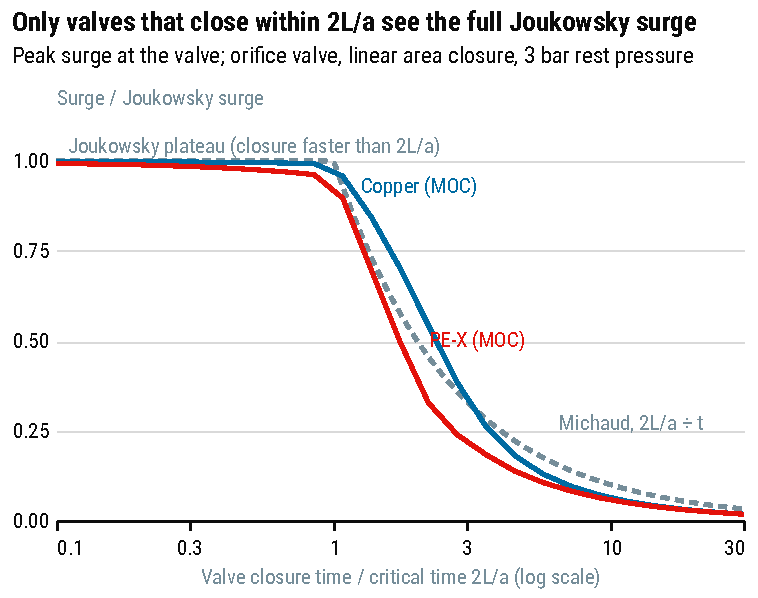
\includegraphics[width=\linewidth]{figures/closure_time.pdf}
  \caption{Peak surge, as a fraction of the Joukowsky value, against closure time measured in units of $2L/a$. The dashed line is Equations~\ref{eq:joukowsky} and \ref{eq:michaud}; the solid lines are the method of characteristics with an orifice valve.}
  \label{fig:closure}
\end{figure}

Figure~\ref{fig:closure} shows the outcome.
Below $t_v \approx T_c$ every closure gives the full Joukowsky surge.
Above it the surge falls roughly as $1/t_v$.
The simulated curve can lie above or below Michaud, depending on how hard the orifice throttles relative to the rest pressure.
\marginnote{The ratio $a v_0 / 2 g H_0$ (Allievi's pipeline constant) measures this. It is larger in copper than in PE-X.}
The model therefore uses the \emph{larger} of the closed-form and simulated values as the design surge.

\begin{figure}
  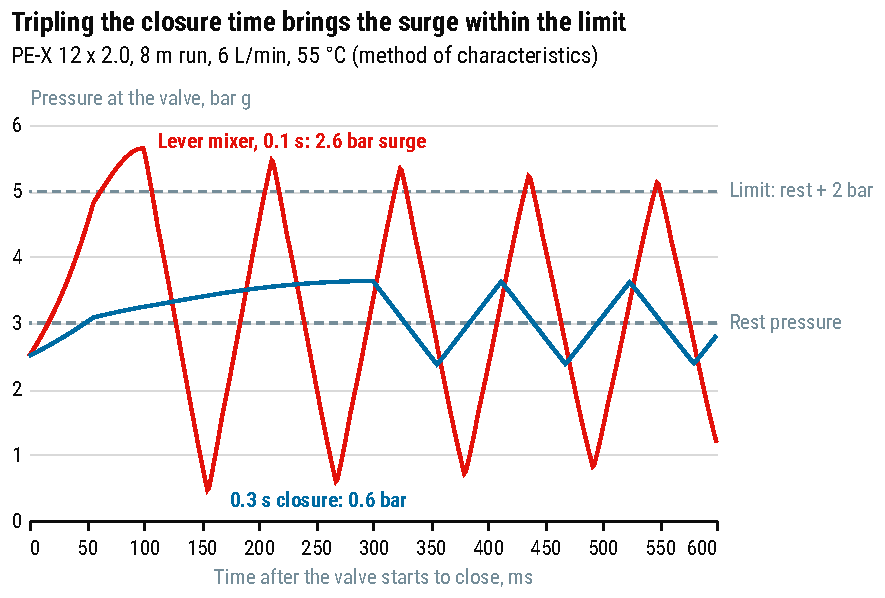
\includegraphics[width=\linewidth]{figures/trace.pdf}
  \caption{Pressure at the valve after closure. Each spike is the wave returning from the reflection point; the period is $4L/a$. Friction damps the oscillation slowly.}
  \label{fig:trace}
\end{figure}

\section{Column separation}

Each high-pressure wave is followed by a low-pressure one of about the same size (Figure~\ref{fig:trace}).
If the pressure falls to the vapour pressure $p_v$ the water column breaks, leaving a vapour cavity.
When the columns rejoin, the impact can exceed the Joukowsky value.\cite[ch.~8]{wylie1993}
The model does not simulate this; it treats any minimum below $p_v$ as a failure.
\marginnote{At \SI{3}{bar} rest pressure this happens once the surge exceeds about \SI{4}{bar}.}

\section{Gas-cushion arresters}

A water hammer arrester places a gas volume, separated from the water by a piston or membrane, next to the valve.
To first order it must absorb the kinetic energy of the column while the pressure rises by no more than the allowed $\Delta p_a$.
Ignoring the energy stored in the pipe wall and the water (which makes the estimate conservative), and with $p$ absolute and gas compressed polytropically with index $n$,
\begin{equation}
  \tfrac12 \rho A L v^2 = \frac{p_0 V_0}{n-1}\left[\left(\frac{p_0+\Delta p_a}{p_0}\right)^{(n-1)/n} - 1\right],
\end{equation}
which tends to $p_0 V_0 \ln\!\left[(p_0+\Delta p_a)/p_0\right]$ as $n\to1$.
The model takes $n = 1.4$ (adiabatic, which needs more volume than isothermal) and a precharge $p_0$ equal to the rest pressure.
The result is a check on scale only; selection should follow the manufacturer's data, or PDI-WH~201 in US practice.\cite{pdiwh201}

\section{Acceptance limits}

\begin{table*}
  \small
  \begin{tabular}{@{}p{0.24\linewidth}p{0.26\linewidth}p{0.46\linewidth}@{}}
    \toprule
    Check & Default & Source \\
    \midrule
    Surge above rest pressure & $\le \SI{2}{bar}$ & Technical rules for drinking water installations (EN 806-2 with DIN 1988-200), as quoted in VDI 6006 \S4.3 \\
    Peak pressure & $\le$ pipe and fitting rating at temperature (\SI{10}{bar} by default) & Water Supply (Water Fittings) Regulations 1999, Sch.~2 paras 3, 5, 12 \\
    Minimum pressure & $> p_v$ & Column separation \\
    Velocity (advisory) & $\le \SI{1.5}{m/s}$ hot & UPC 610.12; DIN 1988-300 allows \SI{2}{m/s} in connection pipes \\
    \bottomrule
  \end{tabular}
  \caption{Checks applied. Any failure of the first three means mitigation is required. Every limit is an input to the model.}
  \label{tab:limits}
\end{table*}

UK and European practice is performance-based: keep the rise within \SI{2}{bar} \citep{en806,din1988,vdi6006}.
The UK Water Fittings Regulations require fittings to resist pressure surges and to withstand 1.5 times the maximum operating pressure \citep{wsr1999}.
US codes are prescriptive: the International Plumbing Code and Uniform Plumbing Code require an arrester to ASSE~1010 wherever quick-closing valves are used \citep{ipc,upc,asse1010}.
Table~\ref{tab:limits} lists the checks.

When mitigation is needed the model reports three remedies.
The first is an arrester at the valve, with the indicative volume above.
The second is the shortest effective closure time that meets the limit, found by bisection on the larger of Michaud and the simulation (the Excel version gives the Michaud estimate).
The third is the largest flow for which even instantaneous closure passes, $\Delta v \le \Delta p_a/(\rho a)$.

\section{Worked example}

A solenoid valve (dishwasher or digital shower, effective closure \SI{20}{ms}) is at the end of \SI{8}{m} of $10\times\SI{0.6}{mm}$ copper.
The flow is \SI{6}{L/min} of water at \SI{55}{\celsius}, and the rest pressure is \SI{3}{bar}.

\begin{fullwidth}
\small
\begin{tabular}{@{}lll@{}}
  \toprule
  Quantity & Working & Result \\
  \midrule
  Bore, area & $D = 10 - 2(0.6) = \SI{8.8}{mm}$; $A = \pi D^2/4$ & \SI{6.08e-5}{m^2} \\
  Velocity & $v = (6/60000)/A$ & \SI{1.64}{m/s} \\
  Water & $\rho = \SI{985.6}{kg/m^3}$, $c = \SI{1546.8}{m/s}$, $K = \rho c^2$ & \SI{2.36}{GPa} \\
  Restraint factor & $2(0.6/8.8)(1.34) + 8.8(1-0.34^2)/9.4$ & $\psi = 1.011$ \\
  Wave speed & $a = 1546.8/\sqrt{1 + 1.011 \times 2.36 \times 8.8/(115.9 \times 0.6)}$ & \SI{1356}{m/s} \\
  Critical time & $2L/a = 16/1356$ & \SI{11.8}{ms} ($< t_v$: slow) \\
  Joukowsky & $\rho a v$ & \SI{22.0}{bar} \\
  Michaud & $2\rho L v/t_v$ & \SI{13.0}{bar} \\
  Simulation & method of characteristics, 20 reaches & \SI{15.8}{bar} \\
  Design surge & larger of the two & \textcolor{econred}{\SI{15.8}{bar} $\gg$ \SI{2}{bar}: mitigation required} \\
  Arrester volume & $\tfrac12 \rho A L v^2 = \SI{0.65}{J}$; $p_0 = \SI{4.01}{bar}$ abs, $n = 1.4$ & $V_0 \approx \SI{5}{ml}$ \\
  Slower valve & surge $\le \SI{2}{bar}$ needs & $t_v \ge \SI{0.13}{s}$ \\
  Lower flow & $\Delta v \le \Delta p_a/\rho a$ & $Q \le \SI{0.55}{L/min}$ \\
  \bottomrule
\end{tabular}
\end{fullwidth}

The peak pressure (\SI{18.8}{bar}) also exceeds the pipe rating, and the following low-pressure wave would separate the column.
In this case an arrester at the appliance valve is the practical answer.

\begin{figure*}
  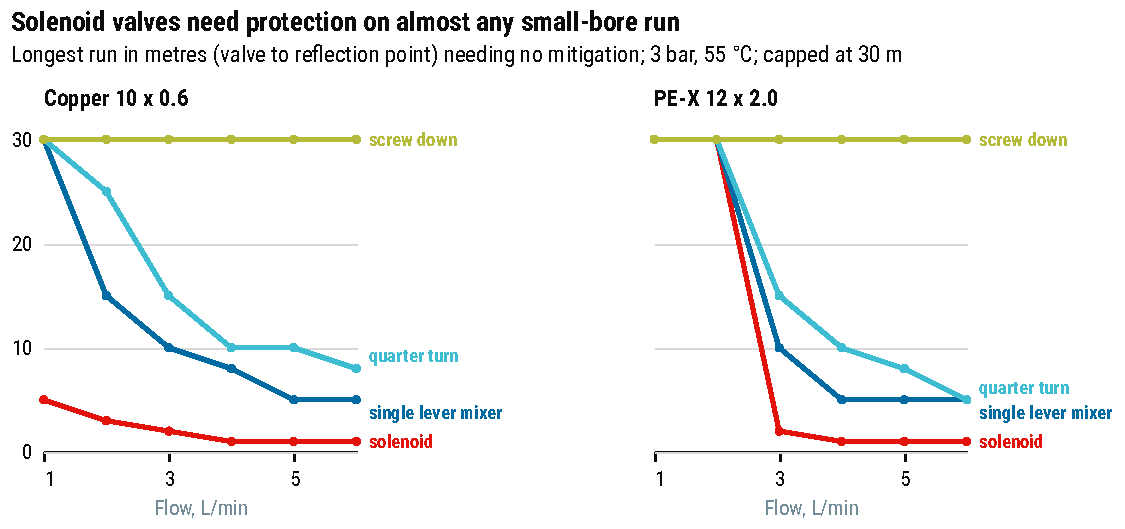
\includegraphics[width=\linewidth]{figures/screening.pdf}
  \caption{Screening results from the model for two common small-bore pipes. Each line is the longest run that needs no mitigation, at \SI{3}{bar} and \SI{55}{\celsius}. The full table for six pipes is in \texttt{results/waterhammer/screening.csv}.}
  \label{fig:screening}
\end{figure*}

\section{What the screening shows}

Figure~\ref{fig:screening} applies the model across the project's design range.
Solenoid valves on small-bore pipe exceed the limit at almost any length once the flow passes 2 to \SI{3}{L/min}.
Lever mixers and quarter-turn taps are acceptable on short runs but fail on long small-bore ones.
Reducing the bore to cut dead-leg volume raises velocity, and so surge.
The two design aims pull against each other, and this model is the check on that trade-off.

\section{Limitations}

The model covers a single pipe ending at a single valve, with steady friction only.
It ignores local losses at fittings, branches and unsteady friction, so a branched network needs a full transient analysis.\cite{chaudhry2014}
Valve closure times are engineering estimates and should be measured where the result is marginal.
Plastic moduli are indicative, and multilayer pipe is treated as a homogenised wall.
Column separation is detected, not simulated.
Trapped air and flexible connections soften real surges, so the results lean conservative.

\bibliographystyle{plainnat}
\bibliography{references}

\end{document}
